\documentclass[aps,prl,onecolumn,notitlepage,showpacs,floatfix,superscriptaddress]{revtex4-1}
\usepackage{dcolumn}
\usepackage{tabularx}
\usepackage{bm}
\usepackage{soul}
\usepackage{amsmath,amssymb}
\usepackage[colorlinks=true,citecolor=blue,urlcolor=blue,linkcolor=blue]{hyperref}
\usepackage{environ}
\usepackage{graphicx}
\usepackage{caption}
\usepackage{subcaption}

\NewEnviron{eqnsplit}{%
\begin{equation}
\begin{split}
  \BODY
\end{split}
\end{equation}
}

\newcommand{\mrm}[1]{\mathrm{#1}}
\newcommand{\ang}{\mathrm{\AA}}
\newcommand{\bmp}{{\bm p}}
\newcommand{\bmk}{{\bm k}}
\newcommand{\bmr}{{\bm r}}

\bibliographystyle{apsrev4-1}

%%%%%%%%%%%%%%%%%%%%%%%%%%%%%%%%%%%%%%%%%%%%%%%%
\begin{document}
\title{Ramsey Interferometry}

\author{Avinash Rustagi}
\date{\today}
%%%%%%%%%%%%%%%%%%%%%%%%%%%%%%%%%%%%%%%%%%%%%%%%
%%%%%%%%%%%%%%%%%%%%%%%%%%%%%%%%%%%%%%%%%%%%%%%%
\maketitle

Ramsey measurement is done for measuring DC magnetic field. In this measurement, first a $\pi/2$ pulse is applied to an initialized qubit. Then, the qubit is left to evolve freely for a fixed time. Following which, another $\pi/2$ pulse is applied and the state of the qubit is projectively readout. 

To begin, let's consider the action of a microwave magnetic field on qubit dynamics. This is important to design the required $\pi/2$ pulse. To do so, let us start with the Hamiltonian for a qubit with an oscillatory magnetic field applied along the x-axis
\begin{equation}
H = \dfrac{\omega_q}{2} \sigma_{11} - \dfrac{\omega_q}{2} \sigma_{00} + \Omega \cos(\omega t +\phi) [\sigma_{10}+\sigma_{01}]
\end{equation}
where $\sigma_{ij} = \vert i \rangle \langle j \vert$. We can solve this problem in the interaction picture by expressing the Hamiltonian as
\begin{equation}
\begin{split}
H &= H_0 + V \\
H_0 &= \dfrac{\omega}{2} \sigma_{11} - \dfrac{\omega}{2} \sigma_{00} \\
V &=\dfrac{\Delta}{2} \sigma_{11} - \dfrac{\Delta}{2} \sigma_{00}+ \Omega \cos(\omega t +\phi) [\sigma_{10}+\sigma_{01}]
\end{split}
\end{equation}
Here $\Delta = \omega_q - \omega$ is the detuning between the microwave field and the qubit splitting. We can now move to the interaction picture with the RWA
\begin{equation}
\begin{split}
H_I &= e^{i H_0 t} V e^{-i H_0 t} \\
&= \dfrac{\Delta}{2} \sigma_{11} - \dfrac{\Delta}{2} \sigma_{00}+ \dfrac{\Omega}{2} e^{i\phi} \sigma_{01} + \dfrac{\Omega}{2} e^{-i\phi} \sigma_{10} \\
&= \dfrac{1}{2} \left[ \begin{array}{cc}
-\Delta & \Omega e^{i\phi} \\ 
\Omega e^{-i\phi} & \Delta
\end{array} \right] 
\end{split}
\end{equation}
In the interaction picture, the evolution of wavefunction is governed by the interaction Hamiltonian. The eigenvalues and eigenvectors for this Hamiltonian is
\begin{equation}
\begin{split}
\lambda_1 &= -\dfrac{1}{2} \tilde{\Omega} \qquad \vert v_1 \rangle = \left[ \begin{array}{c}
\cos(\theta/2)  \\ 
-e^{-i\phi} \sin(\theta/2)
\end{array} \right] \\
\lambda_2 &= +\dfrac{1}{2} \tilde{\Omega} \qquad \vert v_2 \rangle = \left[ \begin{array}{c}
\sin(\theta/2)  \\ 
e^{-i\phi}\cos(\theta/2)
\end{array} \right] 
\end{split}
\end{equation}
where $\tilde{\Omega} = \sqrt{\Omega^2+\Delta^2}$ and $\tan\theta = \Omega/\Delta$. For now, we will restrict to the case where the driving field phase $\phi=0$. The wavefunction in the interaction picture evolves as
\begin{equation}
\vert \Psi_I(t) \rangle = e^{-iH_I t} \vert \Psi_I(0) \rangle
\end{equation}
Lets initialize the qubit to state $\vert \Psi_I(0) \rangle = \vert 0 \rangle$,
\begin{equation}
\vert \Psi_I(0) \rangle = \vert 0 \rangle = \cos(\theta/2) \vert v_1 \rangle + \sin(\theta/2) \vert v_2 \rangle 
\end{equation}
Thus,
\begin{equation}
\begin{split}
\vert \Psi_I(t) \rangle &= e^{-iH_I t} \vert \Psi_I(0) \rangle \\
&= \cos(\theta/2) e^{-i \lambda_1 t} \vert v_1 \rangle + \sin(\theta/2) e^{-i \lambda_2 t} \vert v_2 \rangle
\end{split}
\end{equation}
Therefore, the probability to find the system in the ground state
\begin{equation}
P_0 (t) = \vert \langle 0 \vert \Psi_I(t) \vert^2 = \dfrac{1}{2} [1+\cos\tilde{\Omega}t] + \dfrac{\cos^2\theta}{2} [1-\cos\tilde{\Omega}t]
\end{equation}
and the transition probability to get to the excited state is
\begin{equation}
P_1 (t) = 1-P_0 (t) = \sin^2\theta \sin^2\left( \dfrac{\tilde{\Omega}t}{2}\right) = \dfrac{\Omega^2}{\Omega^2+\Delta^2} \sin^2 \left[\dfrac{\sqrt{\Omega^2+\Delta^2}t}{2} \right]
\end{equation}
The $\pi/2$ pulse is of duration $T$ such that $P_1=1/2$,
\begin{equation}
T = \dfrac{2}{\sqrt{\Omega^2+\Delta^2}} \sin^{-1} \left[\dfrac{\sqrt{\Omega^2+\Delta^2}}{\Omega \sqrt{2}} \right]
\end{equation}
The Ramsey pulse can be modeled in terms of the evolution operator as
\begin{equation}
U_{R} = R_0 (T) F(\tau) R_0(T) 
\end{equation}
where
\begin{equation}
R_0(T) = e^{-i H_I T} = e^{i(\Delta T/2) \sigma_z-i(\Omega T/2) \sigma_x} = \left[ \begin{array}{cc}
\cos\dfrac{A}{2} + i \dfrac{\Delta}{\tilde{\Omega}} \sin\dfrac{A}{2} & -i \dfrac{\Omega}{\tilde{\Omega}} \sin\dfrac{A}{2} \\ 
-i \dfrac{\Omega}{\tilde{\Omega}} \sin\dfrac{A}{2}  & \cos\dfrac{A}{2} - i \dfrac{\Delta}{\tilde{\Omega}} \sin\dfrac{A}{2} 
\end{array}\right]
\end{equation}
where $A = \tilde{\Omega}T$. And the free evolution operator is
\begin{equation}
F(\tau) = \left[ \begin{array}{cc}
e^{i\Delta \tau/2} & 0 \\ 
0 & e^{-i\Delta \tau/2}
\end{array}\right]
\end{equation}
Therefore, the total evolution operator for the Ramsey pulse is
\begin{equation}
U_{R} = \left[ \begin{array}{cc}
\cos\dfrac{A}{2} + i \dfrac{\Delta}{\tilde{\Omega}} \sin\dfrac{A}{2} & -i \dfrac{\Omega}{\tilde{\Omega}} \sin\dfrac{A}{2} \\ 
-i \dfrac{\Omega}{\tilde{\Omega}} \sin\dfrac{A}{2}  & \cos\dfrac{A}{2} - i \dfrac{\Delta}{\tilde{\Omega}} \sin\dfrac{A}{2} 
\end{array}\right] \left[ \begin{array}{cc}
\left(\cos\dfrac{A}{2} + i \dfrac{\Delta}{\tilde{\Omega}} \sin\dfrac{A}{2}\right)e^{i\Delta \tau/2} & -i \dfrac{\Omega}{\tilde{\Omega}} \sin\dfrac{A}{2} e^{i\Delta \tau/2} \\ 
-i \dfrac{\Omega}{\tilde{\Omega}} \sin\dfrac{A}{2} e^{-i\Delta \tau/2} & \left(\cos\dfrac{A}{2} - i \dfrac{\Delta}{\tilde{\Omega}} \sin\dfrac{A}{2} \right)e^{-i\Delta \tau/2}
\end{array}\right]
\end{equation}
The probability to find the system in the excited state would be
\begin{equation}
P_1 = \vert \langle 1 \vert U_R \vert 0 \rangle \vert^2 = \vert (U_R)_{12} \vert^2
\end{equation}
Thus,
\begin{equation}
(U_R)_{12} = -i \dfrac{\Omega}{\tilde{\Omega}}  \left[ \sin A \cos(\Delta \tau/2) - 2 \dfrac{\Delta}{\tilde{\Omega}} \sin^2\dfrac{A}{2} \sin(\Delta \tau/2)\right]
\end{equation}
\begin{equation}
\sin^2 \dfrac{A}{2} = \dfrac{\tilde{\Omega}^2}{2\Omega^2}  \quad \sin A = \dfrac{\tilde{\Omega}}{\Omega} \sqrt{1-\dfrac{\Delta^2}{\Omega^2}}
\end{equation}
Thus,
\begin{equation}
(U_R)_{12} = -i  \left[ \sqrt{1-\dfrac{\Delta^2}{\Omega^2}} \cos(\Delta \tau/2) - \dfrac{\Delta}{\Omega} \sin(\Delta \tau/2)\right] = -i  \left[ \cos\chi \cos(\Delta \tau/2) - \sin\chi \sin(\Delta \tau/2)\right] = -i \cos(\chi+\Delta \tau/2)
\end{equation}
where $\sin\chi = \Delta/\Omega$. Therefore
\begin{equation}
P_1 = \cos^2\left( \dfrac{\Delta \tau}{2} + \chi\right)
\end{equation}
For the case of general phase in the second $\pi/2$ pulse,
\begin{equation}
U_{R} = R_\phi (T) F(\tau) R_0(T) \qquad R_\phi (T) = \left[ \begin{array}{cc}
\cos\dfrac{A}{2} + i \dfrac{\Delta}{\tilde{\Omega}} \sin\dfrac{A}{2} & -i e^{i\phi} \dfrac{\Omega}{\tilde{\Omega}} \sin\dfrac{A}{2} \\ 
-i  e^{-i\phi}\dfrac{\Omega}{\tilde{\Omega}} \sin\dfrac{A}{2}  & \cos\dfrac{A}{2} - i \dfrac{\Delta}{\tilde{\Omega}} \sin\dfrac{A}{2} 
\end{array}\right]
\end{equation}
Consequently,
\begin{equation}
P_1 = \cos^2\left( \dfrac{\Delta \tau}{2} + \chi + \dfrac{\phi}{2}\right)
\end{equation}

\section{Numerical Results}
Solved using the QuTiP toolbox, the Ramsey fringes can be simulated both in the Schrodinger and interaction picture. The driving field is modeled as
\begin{equation}
\vec{H}_{d} (t) = \hat{x} \, H_{d,0} \cos\omega t \, \left[ \Theta(T-t) + \Theta(t-T-\tau) - \Theta(t-2T-\tau)  \right]
\end{equation}
\begin{figure}[hbtp]
 \centering
 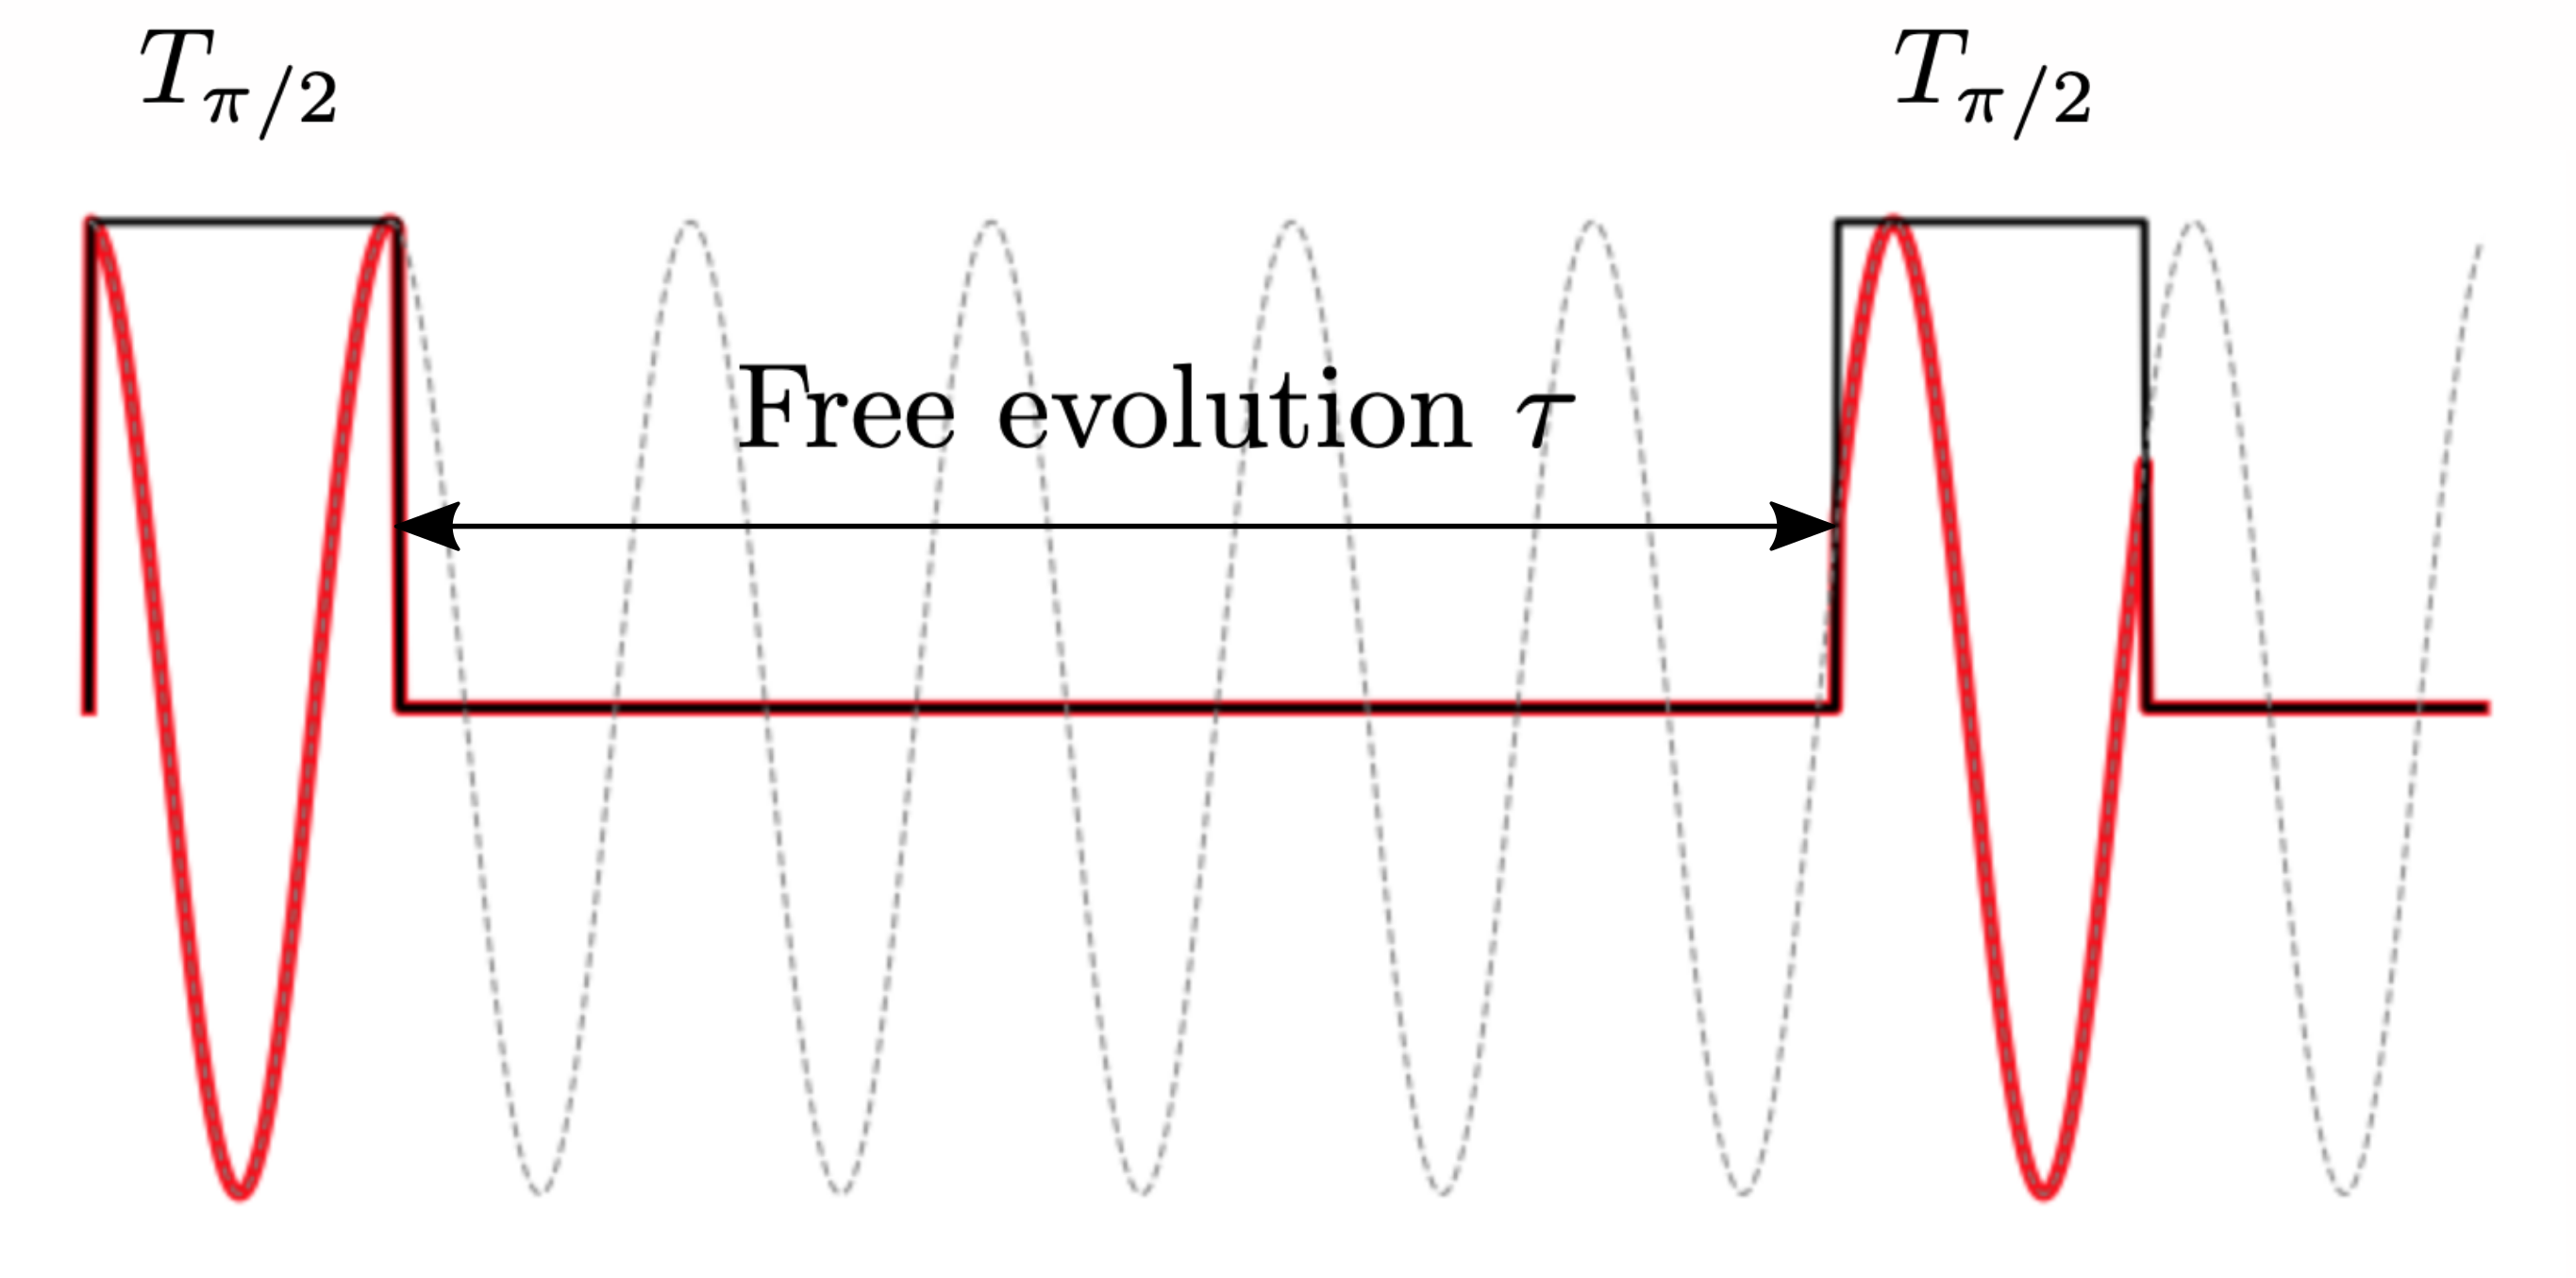
\includegraphics[width=0.4\textwidth]{Ramsey_Pulse.png}
 \caption{Pulse protocol}
 \end{figure}
 
 \begin{figure}[hbtp]
 \centering
 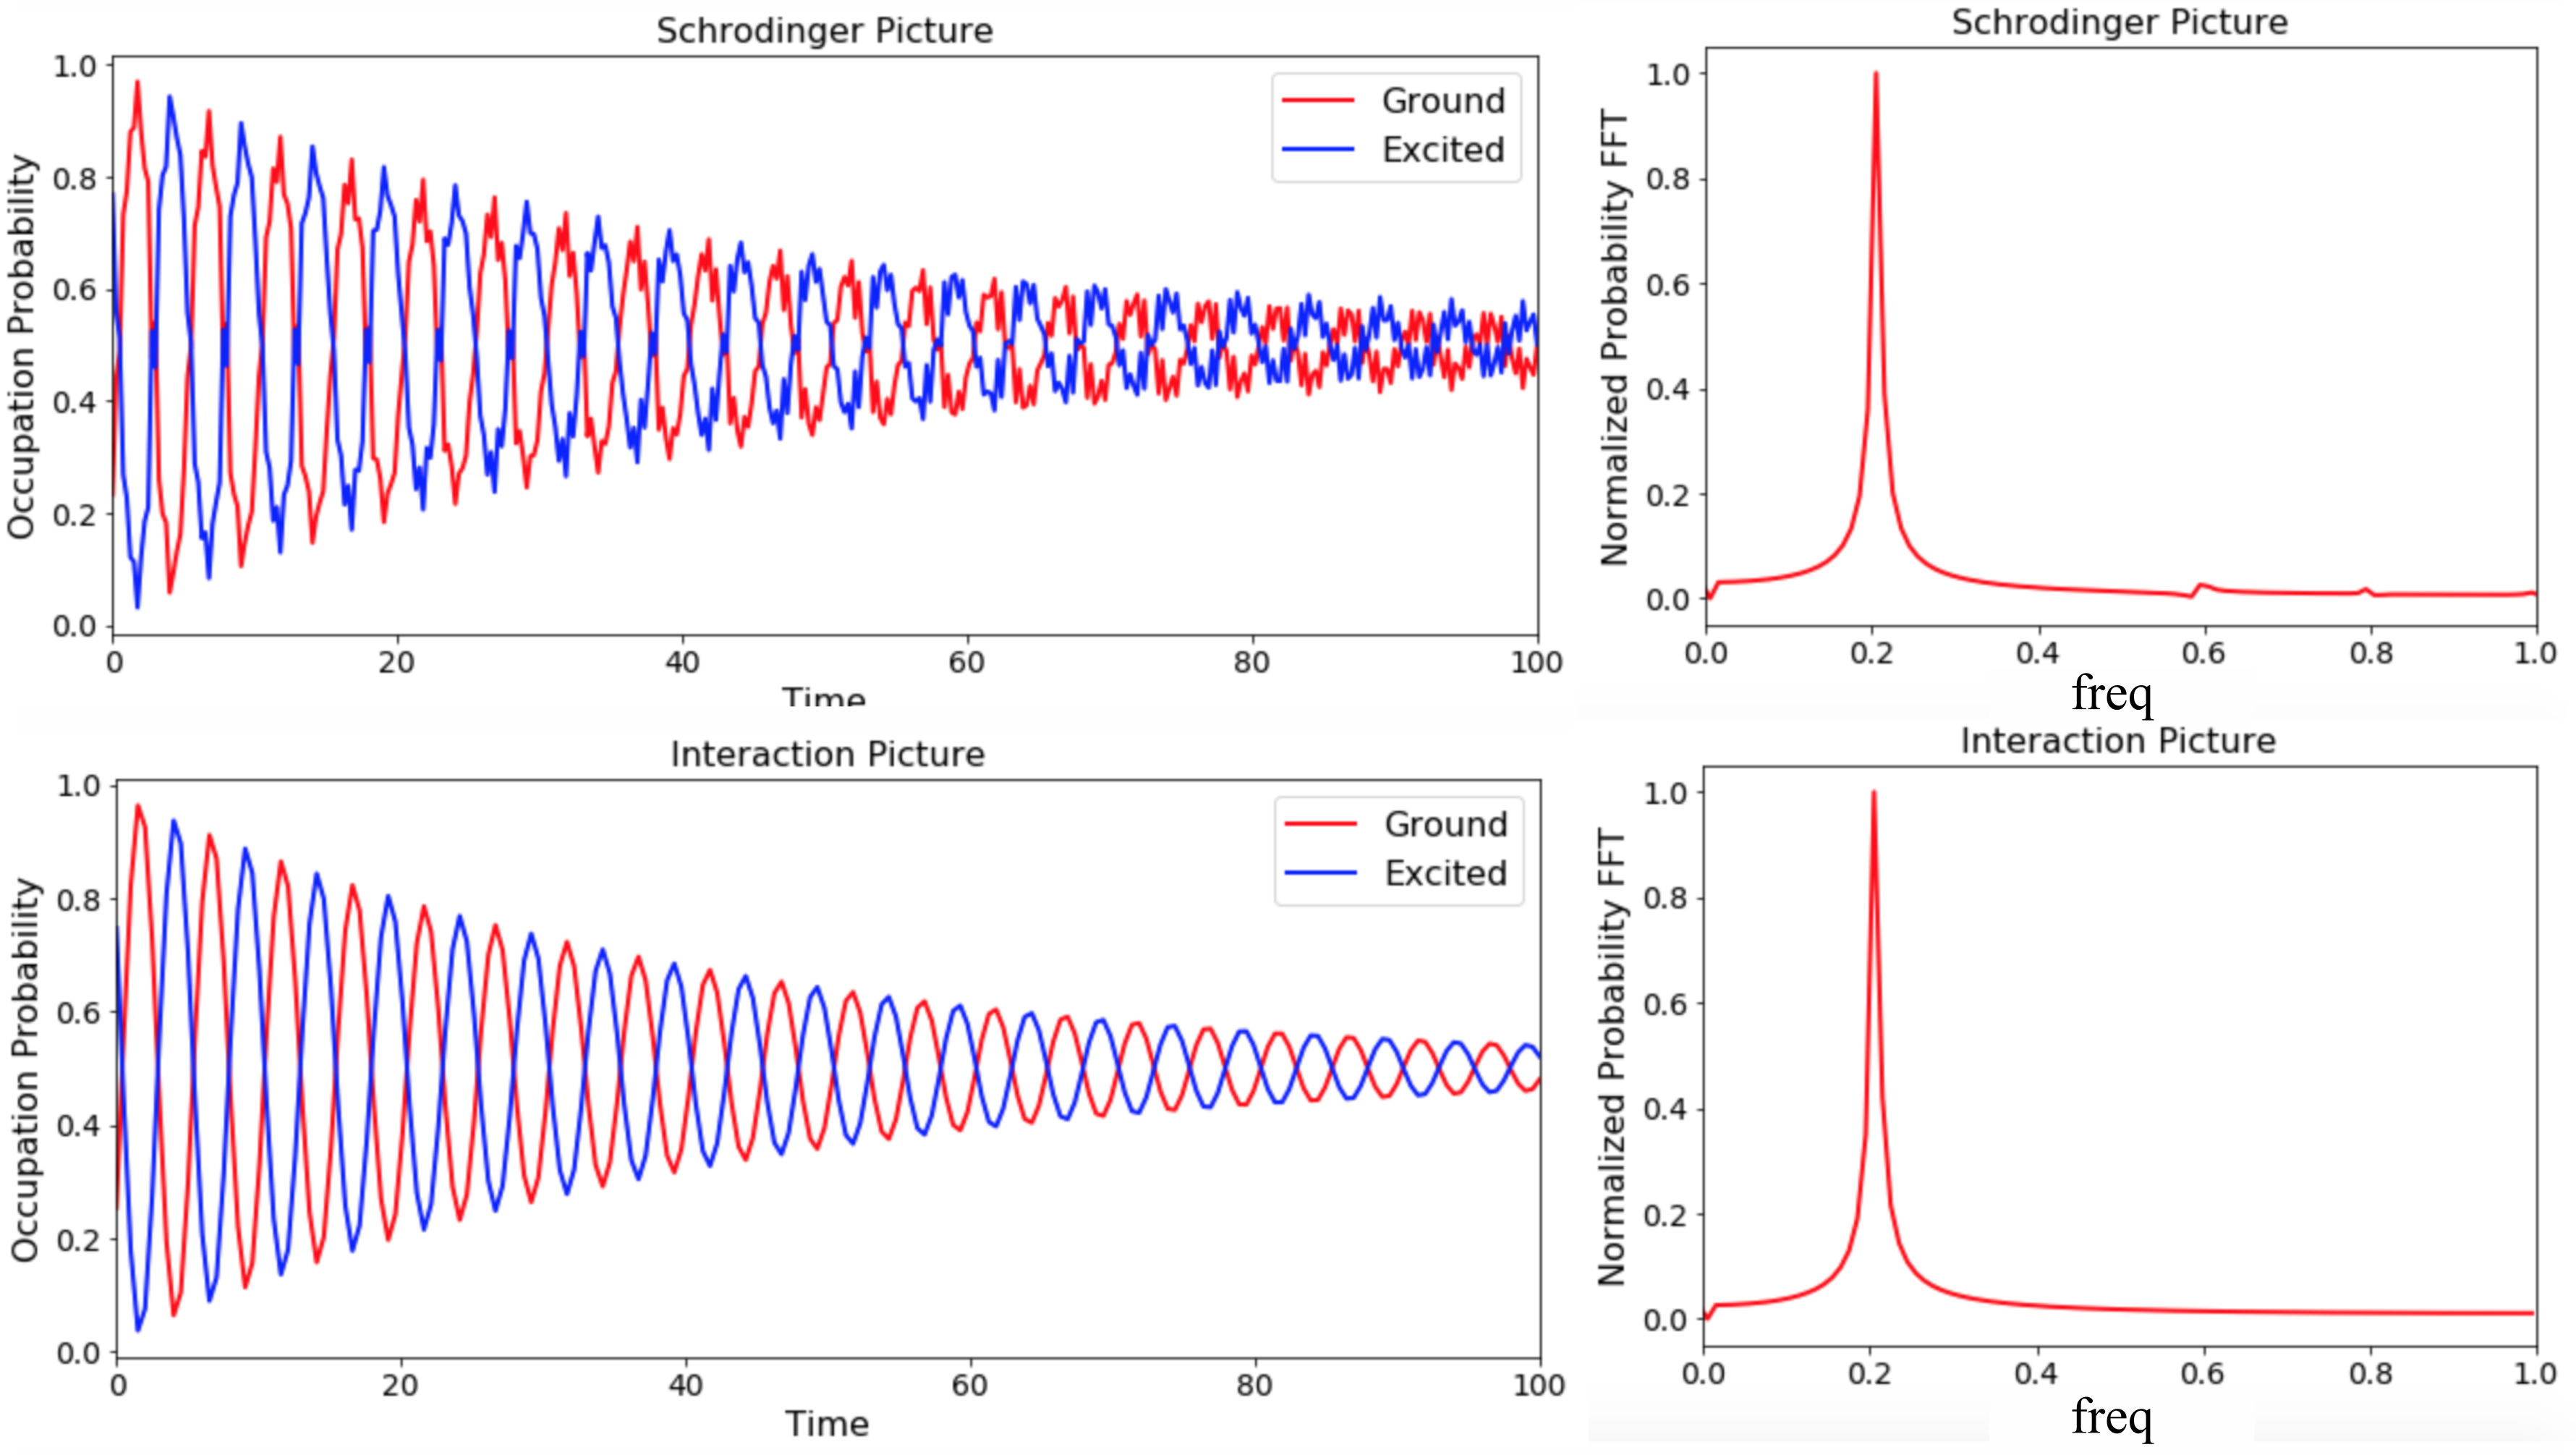
\includegraphics[width=0.9\textwidth]{plots.png}
 \caption{Ramsey fringes. Parameters $\omega_q = 2\pi\times 1$, $\Delta = 2\pi \times 0.2$, $\omega_d = \omega_q-\Delta$, $\Omega = 2\pi \times 0.4$. As seen, the Ramsey fringes oscillate at a frequency set by the detuning between the qubit splitting and the drive frequency.}
 \end{figure}
  
\end{document}